% ============================================================
\chapter{Le Pipeline de la Science des Donn\'ees}
\label{ch:pipeline}
% ============================================================

\section{Qu'est-ce que la science des donn\'ees ?}

\begin{definition}[Science des donn\'ees]
La \textbf{science des donn\'ees} (data science) est une discipline interdisciplinaire qui utilise des m\'ethodes scientifiques, des algorithmes et des syst\`emes pour extraire des connaissances et des informations \`a partir de donn\'ees structur\'ees et non structur\'ees.
\end{definition}

\begin{intuition}
La science des donn\'ees se situe \`a l'intersection de trois domaines :
\begin{itemize}
\item \textbf{Math\'ematiques et Statistiques} : mod\'elisation, inf\'erence, probabilit\'es.
\item \textbf{Informatique} : programmation, algorithmes, bases de donn\'ees.
\item \textbf{Expertise m\'etier} : compr\'ehension du domaine d'application.
\end{itemize}
\end{intuition}

\begin{center}
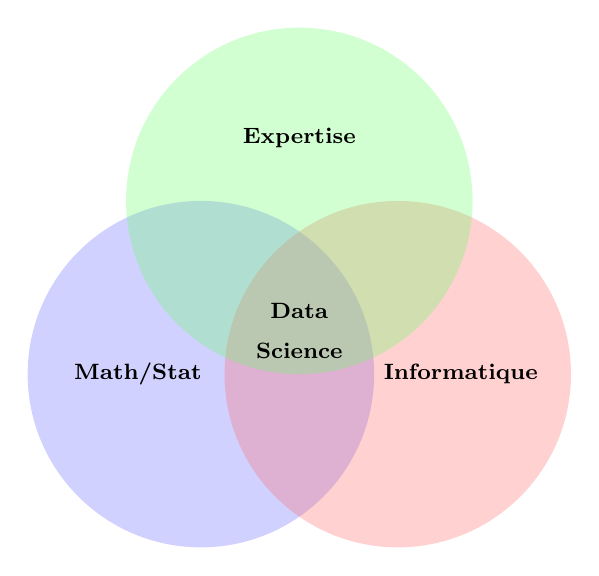
\begin{tikzpicture}
  \begin{scope}[fill opacity=0.3, text opacity=1]
    \fill[blue!60] (0,0) circle (2.2cm);
    \fill[red!60] (2.5,0) circle (2.2cm);
    \fill[green!60] (1.25,2.2) circle (2.2cm);
  \end{scope}
  \node at (-0.8,0) {\footnotesize\textbf{Math/Stat}};
  \node at (3.3,0) {\footnotesize\textbf{Informatique}};
  \node at (1.25,3.0) {\footnotesize\textbf{Expertise}};
  \node at (1.25,0.8) {\footnotesize\textbf{Data}};
  \node at (1.25,0.3) {\footnotesize\textbf{Science}};
\end{tikzpicture}
\end{center}

\section{Le pipeline typique}

Un projet de science des donn\'ees suit g\'en\'eralement un pipeline en plusieurs \'etapes :

\begin{center}
\begin{tikzpicture}[
  block/.style={rectangle, draw, fill=blue!10, rounded corners,
    minimum width=2.8cm, minimum height=0.8cm, align=center, font=\small},
  arr/.style={-{Stealth[length=3mm]}, thick}
]
\node[block] (q) at (0,0) {Question};
\node[block] (d) at (3.5,0) {Donn\'ees};
\node[block] (n) at (7,0) {Nettoyage};
\node[block] (e) at (10.5,0) {Exploration};
\node[block] (m) at (3.5,-1.8) {Mod\'elisation};
\node[block] (v) at (7,-1.8) {\'Evaluation};
\node[block] (c) at (10.5,-1.8) {Communication};
\draw[arr] (q) -- (d);
\draw[arr] (d) -- (n);
\draw[arr] (n) -- (e);
\draw[arr] (e) -- (m);
\draw[arr] (m) -- (v);
\draw[arr] (v) -- (c);
\end{tikzpicture}
\end{center}

\begin{enumerate}
\item \textbf{Formulation de la question} : d\'efinir clairement le probl\`eme.
\item \textbf{Collecte des donn\'ees} : import depuis des fichiers, bases de donn\'ees, API.
\item \textbf{Nettoyage} : traiter les valeurs manquantes, les doublons, les erreurs.
\item \textbf{Exploration} (EDA) : visualiser et r\'esumer les donn\'ees.
\item \textbf{Mod\'elisation} : appliquer des mod\`eles statistiques ou de machine learning.
\item \textbf{\'Evaluation} : mesurer la performance du mod\`ele.
\item \textbf{Communication} : pr\'esenter les r\'esultats de mani\`ere claire.
\end{enumerate}

\section{L'\'ecosyst\`eme Python pour la data science}

\begin{formules}[title=\textbf{Biblioth\`eques essentielles}]
\begin{tabular}{ll}
\toprule
\textbf{Biblioth\`eque} & \textbf{R\^ole} \\
\midrule
\py{numpy} & Calcul num\'erique, tableaux \\
\py{pandas} & Manipulation de donn\'ees tabulaires \\
\py{matplotlib} & Visualisation de base \\
\py{seaborn} & Visualisation statistique \\
\py{scikit-learn} & Apprentissage automatique \\
\py{scipy} & Statistiques et optimisation \\
\bottomrule
\end{tabular}
\end{formules}

\begin{codeblock}[title=\textbf{Python --- Installation et imports}]
\begin{minted}{python}
# Installation (dans un terminal)
# pip install numpy pandas matplotlib seaborn scikit-learn

import numpy as np
import pandas as pd
import matplotlib.pyplot as plt
import seaborn as sns
from sklearn.model_selection import train_test_split
from sklearn.linear_model import LinearRegression

print(f"NumPy:   {np.__version__}")
print(f"Pandas:  {pd.__version__}")
print(f"Seaborn: {sns.__version__}")
\end{minted}
\end{codeblock}

\begin{codeoutput}
\begin{verbatim}
NumPy:   1.26.4
Pandas:  2.2.1
Seaborn: 0.13.2
\end{verbatim}
\end{codeoutput}

\section{Premier exemple complet : le jeu de donn\'ees Iris}

Illustrons le pipeline complet sur le jeu de donn\'ees \textbf{Iris} de Fisher (1936), qui contient 150 mesures de fleurs d'iris r\'eparties en 3 esp\`eces.

\begin{codeblock}[title=\textbf{Python --- Charger et explorer Iris}]
\begin{minted}{python}
from sklearn.datasets import load_iris

# 1. Charger les données
iris = load_iris(as_frame=True)
df = iris.frame
print(df.shape)
print(df.head())
\end{minted}
\end{codeblock}

\begin{codeoutput}
\begin{verbatim}
(150, 5)
   sepal length (cm)  sepal width (cm)  petal length (cm)  petal width (cm)  target
0                5.1               3.5                1.4               0.2       0
1                4.9               3.0                1.4               0.2       0
2                4.7               3.2                1.3               0.2       0
3                4.6               3.1                1.5               0.2       0
4                5.0               3.6                1.4               0.2       0
\end{verbatim}
\end{codeoutput}

\begin{codeblock}[title=\textbf{Python --- Statistiques descriptives}]
\begin{minted}{python}
# 2. Explorer
print(df.describe().round(2))
print(f"\nValeurs manquantes :\n{df.isnull().sum()}")
\end{minted}
\end{codeblock}

\begin{codeoutput}
\begin{verbatim}
       sepal length (cm)  sepal width (cm)  petal length (cm)  petal width (cm)  target
count             150.00            150.00             150.00            150.00  150.00
mean                5.84              3.06               3.76              1.20    1.00
std                 0.83              0.44               1.77              0.76    0.82
min                 4.30              2.00               1.00              0.10    0.00
25%                 5.10              2.80               1.60              0.30    0.00
50%                 5.80              3.00               4.35              1.30    1.00
75%                 6.40              3.30               5.10              1.80    2.00
max                 7.90              4.40               6.90              2.50    2.00

Valeurs manquantes :
sepal length (cm)    0
sepal width (cm)     0
petal length (cm)    0
petal width (cm)     0
target               0
\end{verbatim}
\end{codeoutput}

\begin{codeblock}[title=\textbf{Python --- Visualisation}]
\begin{minted}{python}
# 3. Visualiser
fig, axes = plt.subplots(1, 2, figsize=(12, 5))

# Histogramme
for species in [0, 1, 2]:
    subset = df[df['target'] == species]
    axes[0].hist(subset['petal length (cm)'], alpha=0.6,
                 label=iris.target_names[species], bins=15)
axes[0].set_xlabel('Longueur du pétale (cm)')
axes[0].set_ylabel('Fréquence')
axes[0].legend()

# Nuage de points
for species in [0, 1, 2]:
    subset = df[df['target'] == species]
    axes[1].scatter(subset['sepal length (cm)'],
                    subset['petal length (cm)'],
                    label=iris.target_names[species], alpha=0.7)
axes[1].set_xlabel('Longueur du sépale (cm)')
axes[1].set_ylabel('Longueur du pétale (cm)')
axes[1].legend()
plt.tight_layout()
plt.savefig('ch01_iris_explore.pdf')
plt.show()
\end{minted}
\end{codeblock}

\begin{codeblock}[title=\textbf{Python --- Mod\'elisation simple}]
\begin{minted}{python}
from sklearn.neighbors import KNeighborsClassifier
from sklearn.metrics import accuracy_score

# 4. Modéliser
X = df[['sepal length (cm)', 'sepal width (cm)',
        'petal length (cm)', 'petal width (cm)']]
y = df['target']

X_train, X_test, y_train, y_test = train_test_split(
    X, y, test_size=0.3, random_state=42)

knn = KNeighborsClassifier(n_neighbors=5)
knn.fit(X_train, y_train)
y_pred = knn.predict(X_test)

# 5. Évaluer
print(f"Accuracy : {accuracy_score(y_test, y_pred):.2%}")
\end{minted}
\end{codeblock}

\begin{codeoutput}
\begin{verbatim}
Accuracy : 100.00%
\end{verbatim}
\end{codeoutput}

\section{Types de probl\`emes en data science}

\begin{center}
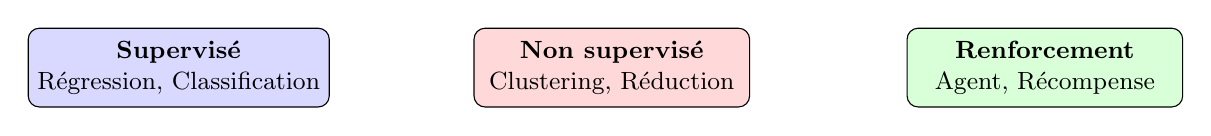
\begin{tikzpicture}[
  box/.style={rectangle, draw, fill=#1!15, rounded corners,
    minimum width=3.5cm, minimum height=1cm, align=center, font=\small},
  arr/.style={-{Stealth}, thick}
]
\node[align=center,box=blue] (sup) at (0,0) {\textbf{Supervis\'e}\\R\'egression, Classification};
\node[align=center,box=red] (unsup) at (5.5,0) {\textbf{Non supervis\'e}\\Clustering, R\'eduction};
\node[align=center,box=green] (semi) at (11,0) {\textbf{Renforcement}\\Agent, R\'ecompense};
\end{tikzpicture}
\end{center}

\begin{itemize}
\item \textbf{Apprentissage supervis\'e} : on dispose d'un label $y$ pour chaque observation $\bm{x}$.
  \begin{itemize}
  \item \emph{R\'egression} : $y \in \R$ (pr\'edire un prix, une temp\'erature).
  \item \emph{Classification} : $y \in \{0,1,\ldots,K-1\}$ (d\'etecter un spam, un cancer).
  \end{itemize}
\item \textbf{Apprentissage non supervis\'e} : pas de label, on cherche des structures (clusters, composantes principales).
\item \textbf{Apprentissage par renforcement} : un agent apprend par essai-erreur dans un environnement.
\end{itemize}

\section{Bonnes pratiques}

\begin{bonnepratique}
\begin{enumerate}
\item \textbf{Reproductibilit\'e} : fixer les graines al\'eatoires (\py{random_state=42}), versionner le code.
\item \textbf{S\'eparation train/test} : ne jamais \'evaluer sur les donn\'ees d'entra\^inement.
\item \textbf{Documentation} : commenter le code, noter les hypoth\`eses.
\item \textbf{It\'eration} : commencer simple, complexifier progressivement.
\end{enumerate}
\end{bonnepratique}

\begin{attention}
Ne jamais regarder les donn\'ees de test avant d'avoir finalis\'e son mod\`ele. Le \emph{data leakage} (fuite de donn\'ees) est l'erreur la plus courante et la plus dangereuse en data science.
\end{attention}

\section{Exercices}

\begin{exercice}[$\star$]
Charger le jeu de donn\'ees \py{load_wine()} de scikit-learn. Afficher ses dimensions, les noms des variables et les statistiques descriptives.
\end{exercice}

\begin{exercice}[$\star$]
Sur le jeu Iris, cr\'eer un nuage de points (\emph{scatter plot}) de la largeur du s\'epale en fonction de la longueur du s\'epale, color\'e par esp\`ece.
\end{exercice}

\begin{exercice}[$\star\star$]
Appliquer un classifieur $k$-plus proches voisins au jeu Wine avec $k=3,5,7$. Comparer les pr\'ecisions sur un jeu de test de 30\%.
\end{exercice}

\begin{exercice}[$\star\star$]
\'Ecrire une fonction \py{pipeline_complet(dataset, k)} qui charge un jeu de donn\'ees scikit-learn, le divise en train/test, entra\^ine un KNN avec $k$ voisins et retourne l'accuracy.
\end{exercice}

\begin{formules}[title=\textbf{R\'esum\'e du chapitre}]
\begin{itemize}
\item La science des donn\'ees suit un pipeline : Question $\to$ Donn\'ees $\to$ Nettoyage $\to$ Exploration $\to$ Mod\'elisation $\to$ \'Evaluation $\to$ Communication.
\item L'\'ecosyst\`eme Python offre des outils puissants : \py{pandas}, \py{matplotlib}, \py{scikit-learn}.
\item Trois grandes familles : supervis\'e, non supervis\'e, renforcement.
\item R\`egles d'or : reproductibilit\'e, s\'eparation train/test, commencer simple.
\end{itemize}
\end{formules}
